% Intestazione
\fancyhead[L]{Diario della riunione} % Testo a sinistra


\section{Diario della riunione}

\begin{itemize}
    \item \lipsum[1]
    \begin{itemize}
        \renewcommand{\labelitemii}{--}
        \item Item 1
        \item Item 2
        \item Item 3
    \end{itemize}
    \item E' stata redatto il \emph{diagramma delle classi}, rappresentato in Figura \ulref{fig:immagine}.
    \begin{figure}[h]
      \centering
      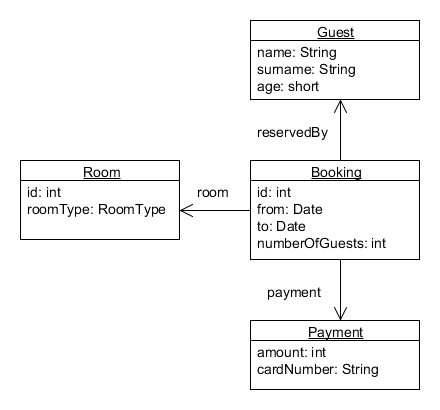
\includegraphics[width=0.5\textwidth]{Model-class-diagram.png}
      \caption{Diagramma delle classi del modello}
      \label{fig:immagine}
    \end{figure}
\end{itemize}